% !TEX root = ../main.tex
\section{Findings in Specific Subgroups}

  In this section the presentation of results will be focused on different user types. Each part will include the same aspects of the patterns; pattern length, pattern creation time, and pattern strength. For some of the user types extra pattern characteristics are included if there are some extra interesting results. 

	\subsection{Gender}

    Gender are divided into male and female participants. For each of the representations, the results will be presented with respect to pattern type and gender. 

    \subsubsection{Average pattern creation time}

    Figure \ref{fig:avgcreationtimegender} shows the average creation time in seconds for both genders. Male participants has in general a higher average creation time than females. The average creation time for shopping account and smartphones are about the same for both genders, while bank has the highest average creation time for both genders. 

    \begin{figure}[H]
      \centering
      \subfigure[Male]{
        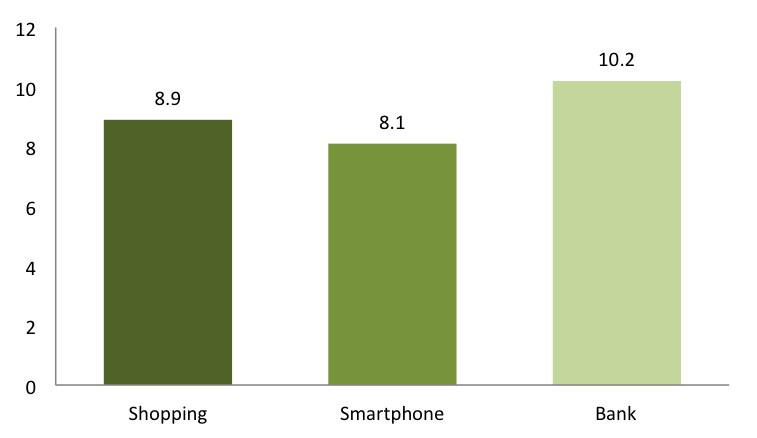
\includegraphics[width=0.45\textwidth]{pics/analysis/creationtime-gender-male.png}
        \label{fig:avgcreationtimemale}
      }
      \subfigure[Female]{
        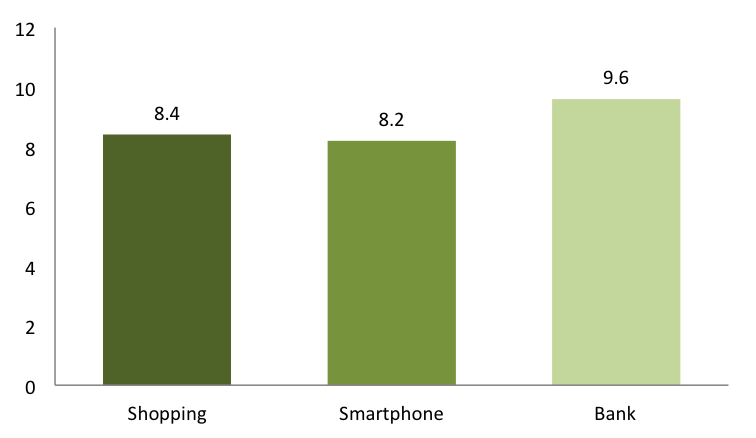
\includegraphics[width=0.45\textwidth]{pics/analysis/creationtime-gender-female.png}
        \label{fig:avgcreationtimefemale}
      }
      \caption{Average pattern creation time for gender}
      \label{fig:avgcreationtimegender}
    \end{figure}

    \clearpage
    \subsubsection{Average pattern length}

    Figure \ref{fig:avgpatternlengthmale} and \ref{fig:avgpatternlengthfemale} shows the pattern length for male and female participants respectively. For male participants there are a slightly difference between the average length of patterns created for shopping and smartphones where the smartphone has the shortest average length of 5.47. The patterns created for banking account has the longest average length of 6.09. Female participants have created about the same length for both shopping and smartphone, while bank has a slightly longer average length than the others. Comparing the longest length for both genders, both have the longest length for banking account and both genders have the the shortest average length for smartphone. In general, the patterns created by male participants have an longer average length than patterns created by female participants. 

    \begin{figure}[H]
    	\centering
    	\subfigure[Male]{
    		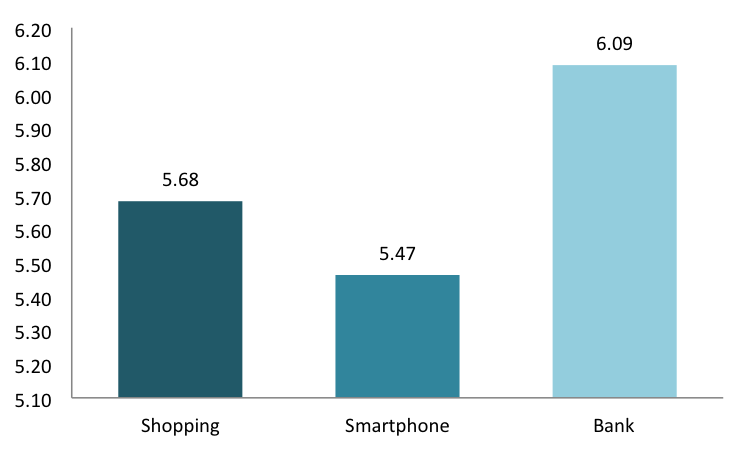
\includegraphics[width=0.45\textwidth]{pics/analysis/avgpatternlength-gender-male.png}
    		\label{fig:avgpatternlengthmale}
    	}
    	\subfigure[Female]{
    		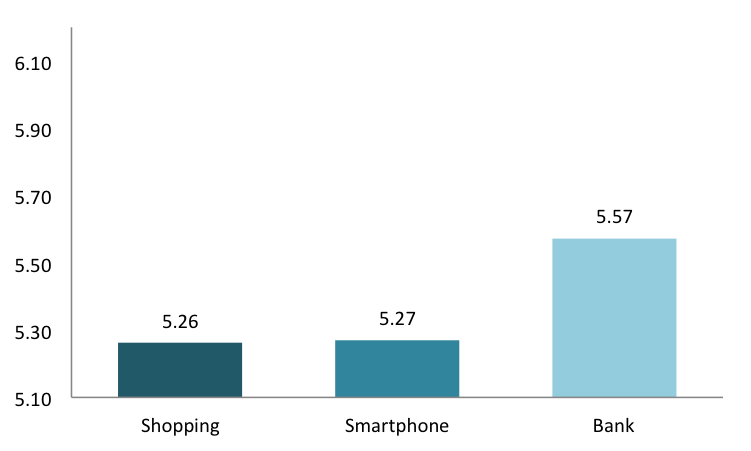
\includegraphics[width=0.45\textwidth]{pics/analysis/avgpatternlength-gender-female.png}
    		\label{fig:avgpatternlengthfemale}
    	}
    	\caption{Average pattern length for gender}
    	\label{fig:avgpatternlengthgender}
    \end{figure}

    \subsubsection{Pattern length distribution}

    Figure \ref{fig:avgpatterndistgender} shows the pattern length distribution for both genders. The differences between the genders are noticeable in the endpoints, e.g. patterns with length 4 and 9, of the distribution. The male participants have a higher frequency of patterns with a longer length, while the female participants have a higher frequency of patterns with a short length. The average number of patterns created with the length 5-8 are about the same for both genders. It is noticeable that there are few occurences of patterns with length 8. 

    \begin{figure}[H]
    	\centering
    	\subfigure[Male]{
    		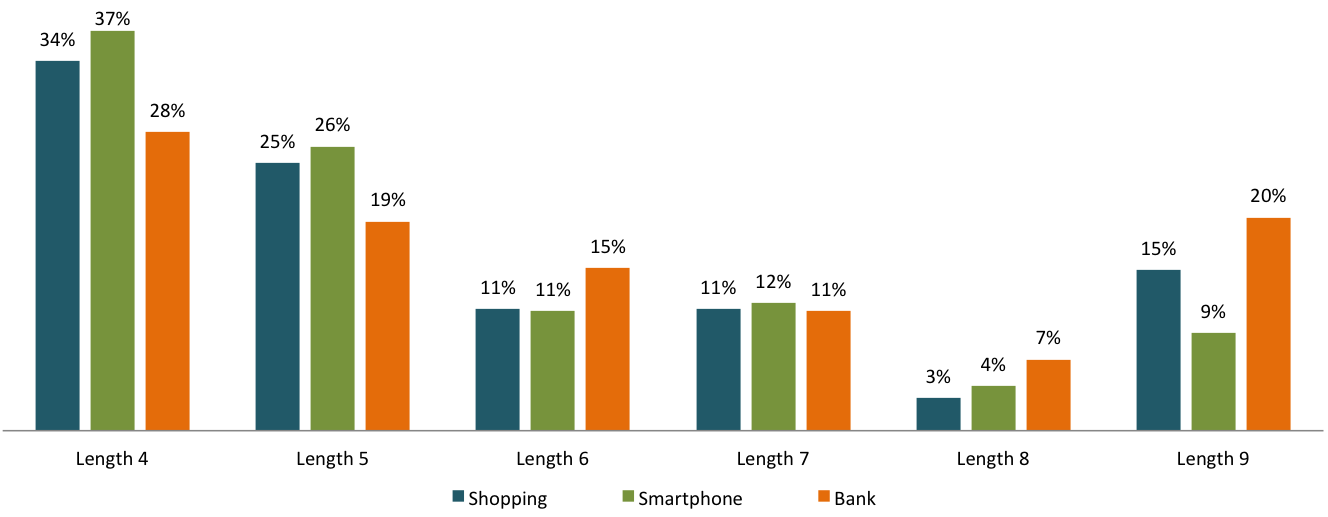
\includegraphics[width=1.0\textwidth]{pics/analysis/patterndist-gender-male.png}
    		\label{fig:avgpatternlengthdistmale}
    	}
    	\subfigure[Female]{
    		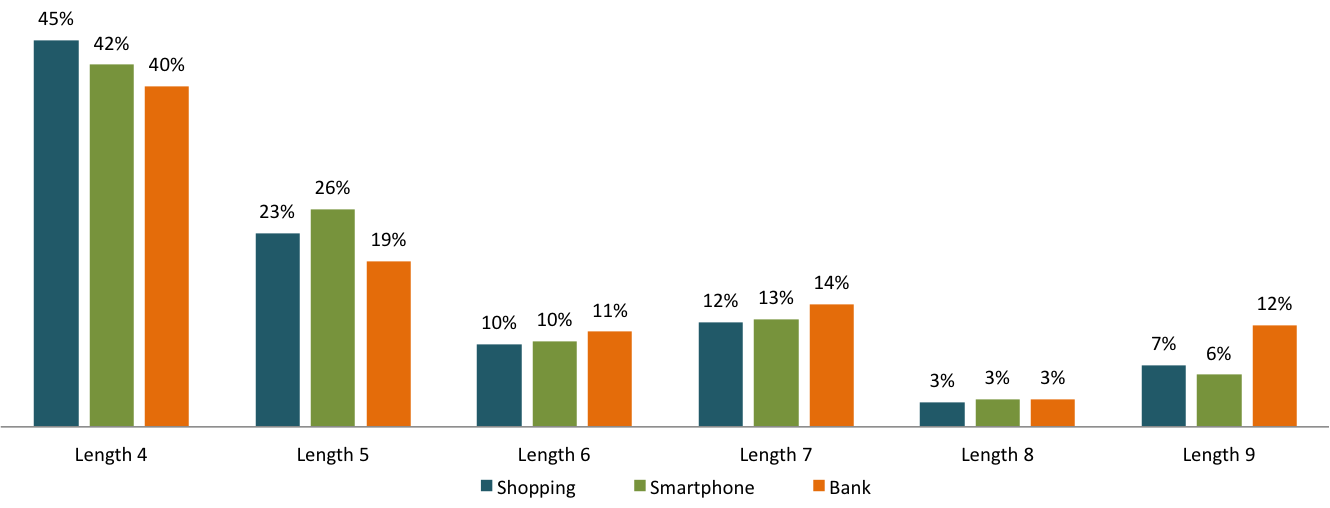
\includegraphics[width=1.0\textwidth]{pics/analysis/patterndist-gender-female.png}
    		\label{fig:avgpatternlengthdistfemale}
    	}
    	\caption{Average pattern length distribution for gender}
    	\label{fig:avgpatterndistgender}
    \end{figure}

    \subsubsection{Pattern complexity}

    Table \ref{tab:gendertrength} shows the patterns strength for the three pattern types for both genders. Patterns created by female participants have the characteristics of infrequent use of both intersections and overlaps for all types. The patterns created by female participants for do not have a single pattern including an overlap.

    The highest strength score are reached for all pattern types for male participants. The pattern strength for patterns created by female participant only reaches a maximum strength of 40.072, that is lower that the maximum patter score in the dataset. The the patterns with the lowest pattern strength are patterns created for smartphones by female participants, only reaching a total strength score of 32.078. 

    \begin{table}[H]
      \centering
      \begin{tabular}{l || l | l || l | l || l | l }
        \hline
         & \multicolumn{2}{c||}{\bf Shopping} & \multicolumn{2}{c||}{\bf Smartphone} &\multicolumn{2}{c}{\bf Bank} \\ \hline
        {\bf Parameters}   & {\bf Male} & {\bf Female} & {\bf Male} & {\bf Female} & {\bf Male} & {\bf Female}\\ \hline
        \#Patterns         & 529    & 278    & 529    & 278    & 529    & 278    \\
        Avg. Size          & 5.684  & 5.263  & 5.465  & 5.270  & 6.089  & 5.572  \\
        Avg. Length        & 5.225  & 4.687  & 5.034  & 4.720  & 5.927  & 5.154  \\
        \#Intersections    & 147    & 20     & 120    & 23     & 284    & 69     \\
        Avg. Intersections & 0.278  & 0.072  & 0.227  & 0.082  & 0.537  & 0.248  \\
        \#Overlaps         & 13     & 1      & 12     & 0      & 16     & 3      \\
        Avg. Overlaps      & 0.025  & 0.04   & 0.023  & 0      & 0.030  & 0.011  \\ \hline
        Avg. Strength      & 14.127 & 12.062 & 13.221 & 12.122 & 16.398 & 13.744 \\ 
        Min strength       & 6.340  & 6.340  & 6.340  & 6.340  & 6.340  & 6.340  \\
        Max strength       & 44.442 & 32.950  & 44.442 & 32.078 & 44.442 & 40.072 \\ \hline
      \end{tabular}
      \caption{Pattern strength and gender }
      \label{tab:gendertrength}
    \end{table}

	\subsection{Age}

    The participants are divided into seven age intervals.

    \subsubsection{Average pattern creation time}
    Figure \ref{fig:patterncreationtimeage} is the average creation time for each pattern type by the different age groups. In general, patterns created for banking account have the highest average creation time across the different age groups. The graph also seems to slightly increase the average creation time as the age increases. It is noticeable that the creation time for smartphone patterns differs from the two other pattern types, especially for the younger participants where pattern creation time for smartphone are significant lower (participants with age between 16 and 24).

    %Figure: pattern creation time by gender
    \begin{figure}[H]
      \centering
      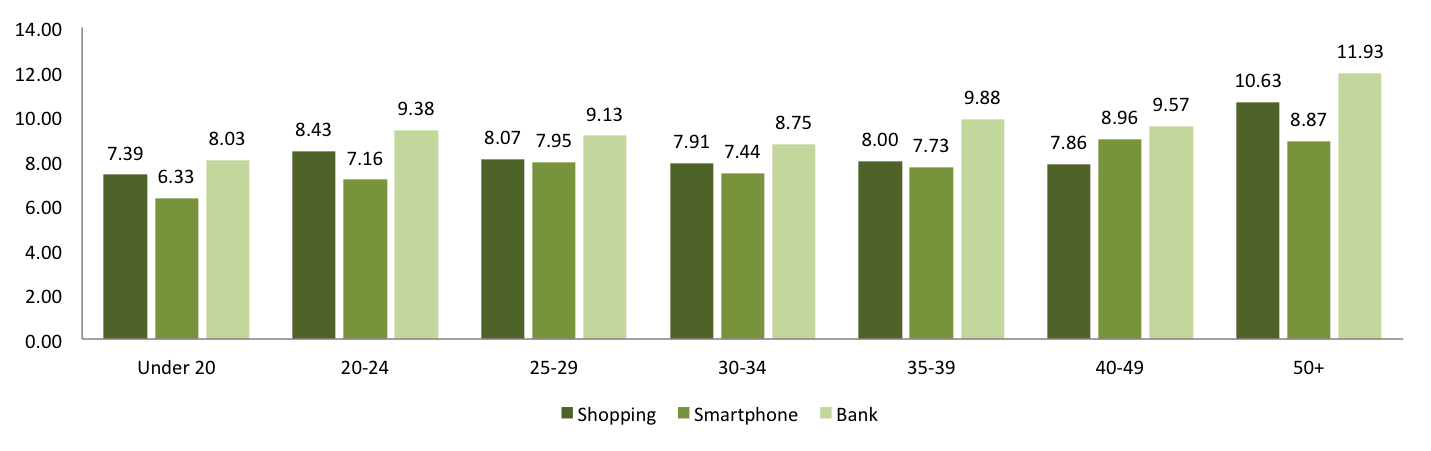
\includegraphics[width=\textwidth]{pics/analysis/creationtime-age.png}
      \caption{Pattern creation time by age}
      \label{fig:patterncreationtimeage}
    \end{figure}

    \clearpage
    \subsubsection{Average pattern length}
    Figure \ref{fig:patternlengthage} shows the pattern length for the three pattern types by the different age groups. In the graph, the average pattern length goes slightly down as the age increases. As the age increase the average length of the all pattern types evens out, meaning that the most significant difference in pattern length between the pattern types are found in the youngest participants.

    %Figure: Average pattern length by age
  	\begin{figure}[H]
	    \centering
	    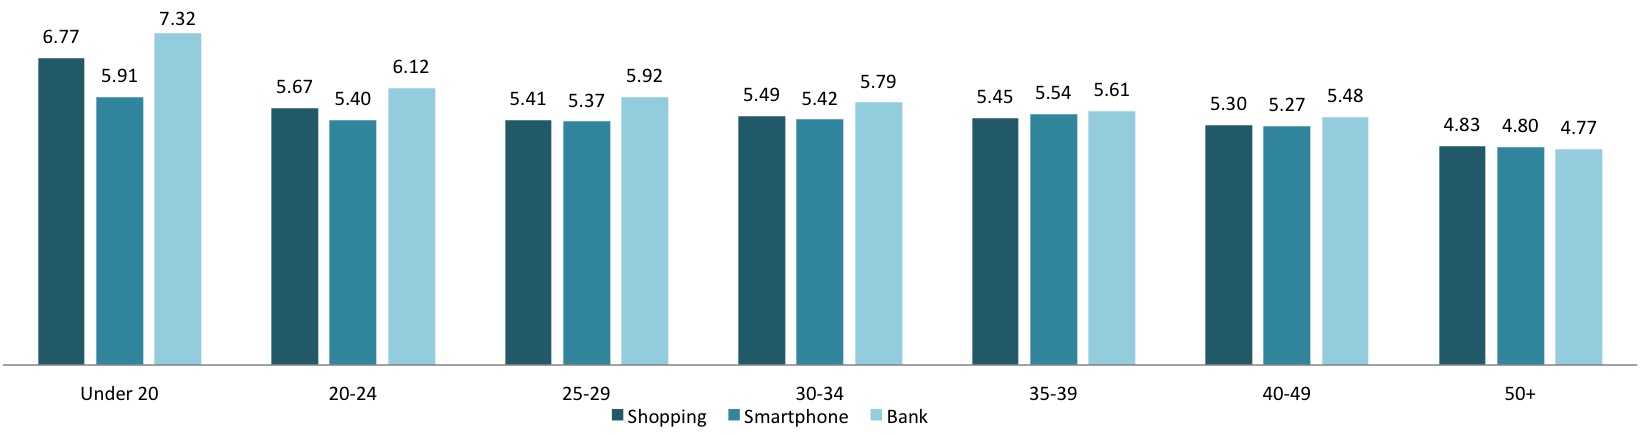
\includegraphics[width=\textwidth]{pics/analysis/avgpatternlength-age.png}
	    \caption{Pattern length by age}
	    \label{fig:patternlengthage}
  	\end{figure}

    \subsubsection{Pattern complexity}
    To be able to illustrate the pattern strength for all age groups the data are shorten down to just visualize the pattern strength of each pattern type created by the different age groups. As mentioned earlier, the younger the longer patterns are noticed to be created. The same is with the strength. The youngest age group have about twice as hight average pattern strength than the oldest age group. As the age goes up, the strength for the different age groups also evens out. In general, bank have the highest average strength score while patterns created for smartphones have the lowest average strength score.

    %Figure: pattern strength based on age
    \begin{figure}[H]
      \centering
      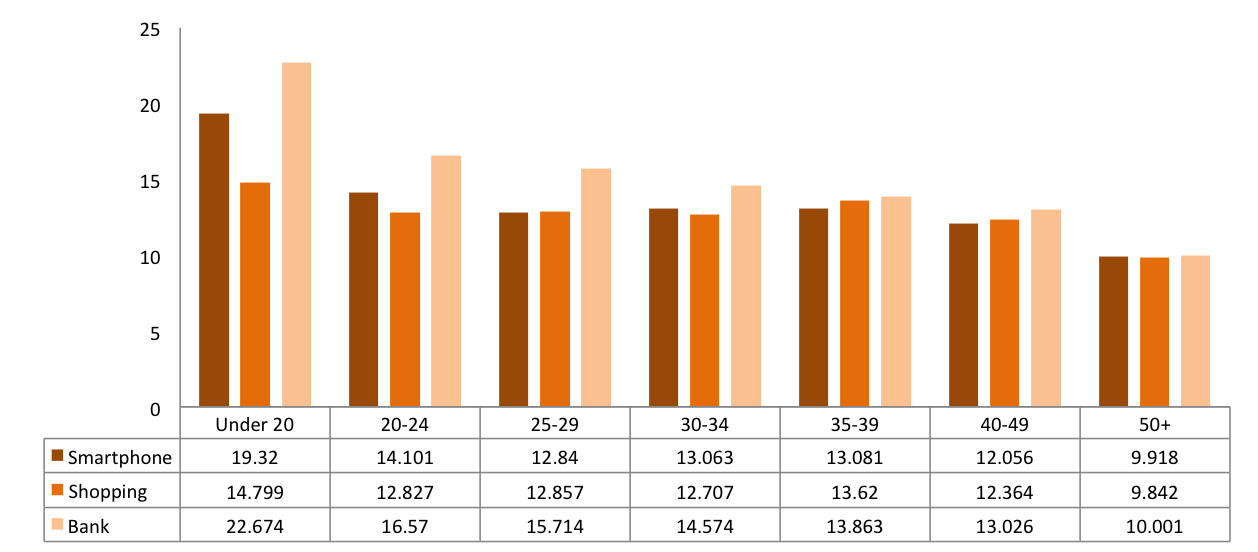
\includegraphics[width=\textwidth]{pics/analysis/strengthagedist.png}
      \caption{Pattern strength and age distribution}
      \label{fig:strengthagedist}
    \end{figure}

	\subsection{Handedness}
		% Kan her dra inn noe om hvilken hånd og finger som er brukt. 

    \subsubsection{Average pattern creation time}
      Figure \ref{fig:avgcreationtimehandedness} is the average creation time for patterns with respect to the handedness of the respondents. A participant can either be left or right handed. By looking at the graph, right-handed respondents has a lover average creation time than left-handed respondents. The only exception is the patterns created for smartphones where left-handed respondents have a slightly higher average creation time. 
      For both left-handed and right-handed respondents, the average creation time for the banking account have the highest average creation among the three pattern types. 

      %Figure: Average pattern creation time for handednes
      \begin{figure}[H]
        \centering
        \subfigure[Right-handed]{
          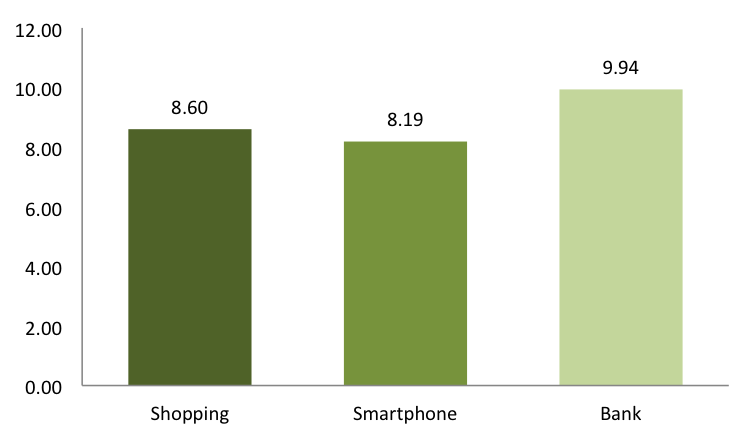
\includegraphics[width=0.45\textwidth]{pics/analysis/creationtime-handedness-right.png}
          \label{fig:avgcreationtimeright}
        }
        \subfigure[Left-handed]{
          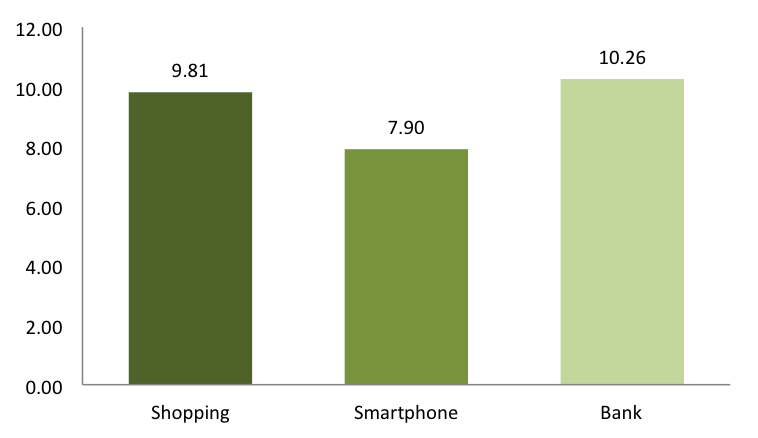
\includegraphics[width=0.45\textwidth]{pics/analysis/creationtime-handedness-left.png}
          \label{fig:avgcreationtimeleft}
        }
        \caption{Average pattern creation time for handedness}
        \label{fig:avgcreationtimehandedness}
      \end{figure}

    \subsubsection{Average pattern length}
      Figure \ref{fig:avgpatternlengthright} and \ref{fig:avgpatternlengthhandedness} shows the average pattern length for pattern created by left- and right-handed respectively. In general, both left- and right-handed respondents have about the same average pattern length. One exception is the patterns created for smartphones where there is a slightly indication that left-handed people create shorter patterns than right-handed people. The patterns getting the highest average length is the patterns created for banking accounts. 

      %Figure: Average pattern length for handedness
      \begin{figure}[H]
      	\centering
      	\subfigure[Right-handed]{
      		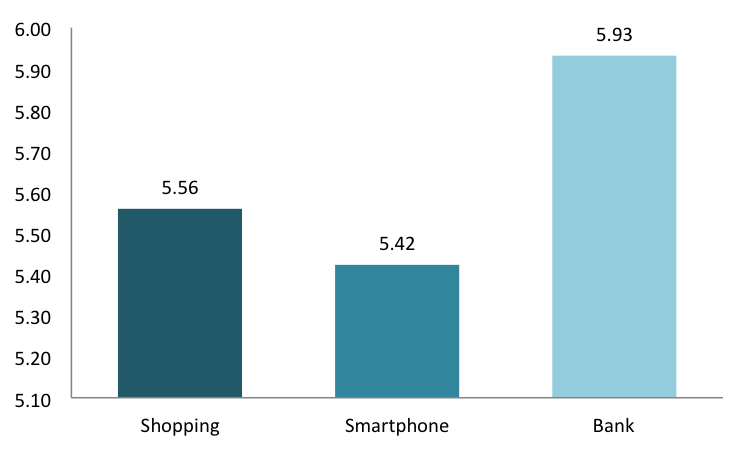
\includegraphics[width=0.45\textwidth]{pics/analysis/avgpatternlength-handedness-right.png}
      		\label{fig:avgpatternlengthright}
      	}
      	\subfigure[Left-handed]{
      		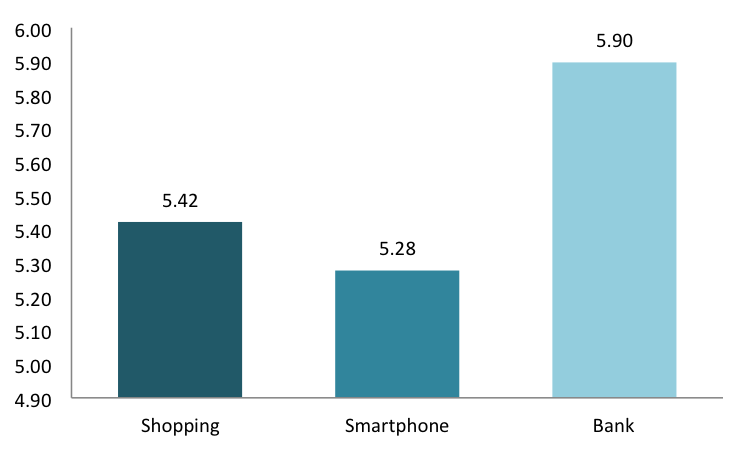
\includegraphics[width=0.45\textwidth]{pics/analysis/avgpatternlength-handedness-left.png}
      		\label{fig:avgpatternlengthleft}
      	}
      	\caption{Average pattern length for handedness}
      	\label{fig:avgpatternlengthhandedness}
      \end{figure}

    \subsubsection{Pattern length distribution}
      Figure \ref{fig:avgpatterndisthandedness} shows the pattern length distribution for both right- and left-handed respondents. The selection of pattern length seems to have no significant difference beside that left-handed respondents have a tendency of have a higher frequency of patterns with length 4 than right-handed respondents. 
      It is also noticeable that the frequency of patterns tends to go down as the pattern length goes up. The only exception are patterns with length 8 where patterns with length 7 and 9 have a higher frequency.

      A pattern length of 4 and 5 can be considered as a short pattern whereas the minimum pattern length is 4. By looking at the number of patterns with the minimum length 4, 45\% of the left-handed respondents created a pattern of length 4 for smartphone that is close to half of the respondents. In total, 70\% of all left-handed respondent created a pattern of length 4 or 5 for smartphone. 65\% of the patterns created for smartphones by Right-handed respondents is of length 4 or 5, a slightly lower percentage than for left-handed respondents. Compared to patterns created for banking accounts, there are only 51\% and 52\% of the patterns having a length of 4 or 5 for right- and left-handed respondents respectively. This is difference of 15\% and 20\% for right- and left-handed respondents between patterns created for smartphone and banking accounts with length 4 and 5.  

      %Figure: Pattern length dist handedness
      \begin{figure}[H]
      	\centering
      	\subfigure[Right-handed]{
      		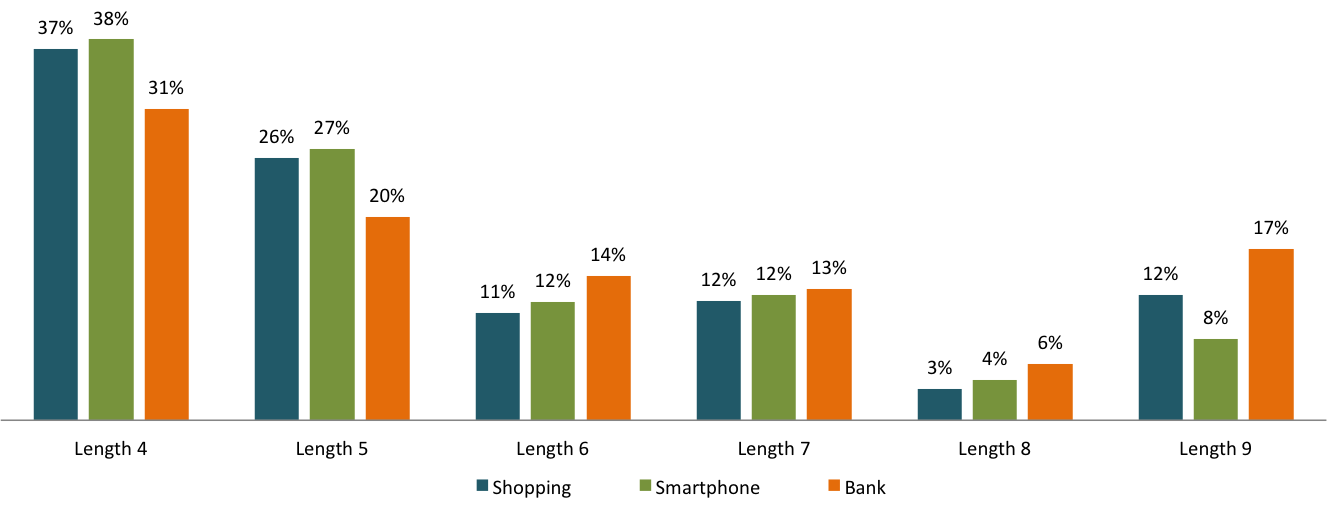
\includegraphics[width=1.0\textwidth]{pics/analysis/patterndist-handedness-right.png}
      		\label{fig:avgpatternlengthdistright}
      	}
      	\subfigure[Left-handed]{
      		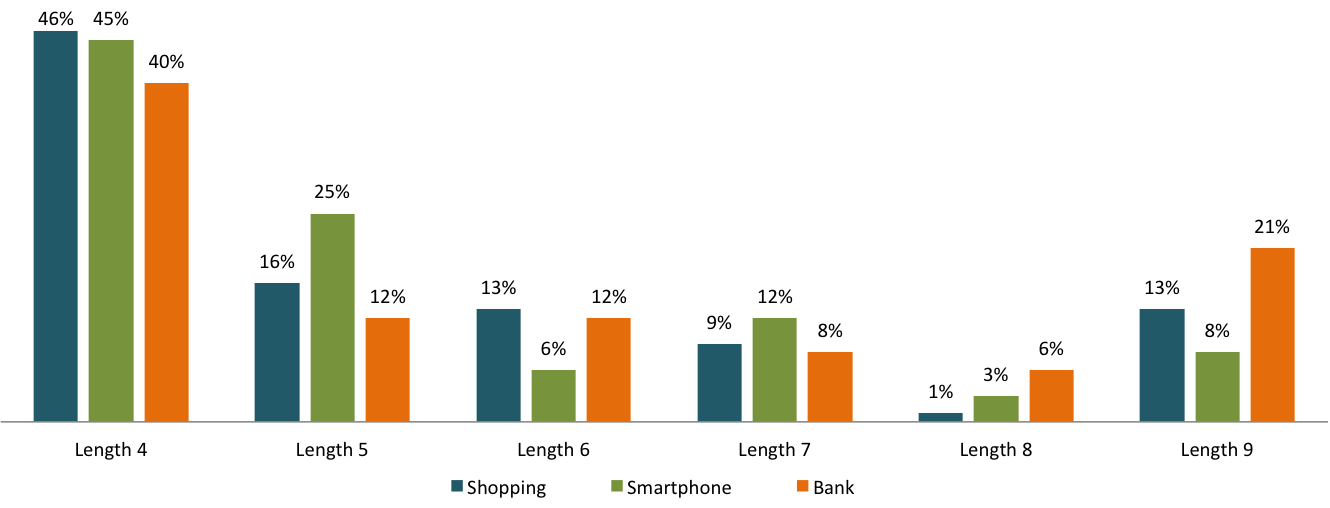
\includegraphics[width=1.0\textwidth]{pics/analysis/patterndist-handedness-left.png}
      		\label{fig:avgpatternlengthdistleft}
      	}
      	\caption{Average pattern length distribution for handedness}
      	\label{fig:avgpatterndisthandedness}
      \end{figure}

    \subsubsection{Pattern complexity}

      Table \ref{tab:handednessstrength} is the pattern strength for each pattern type with respect to the handedness of the respondents, including a overview of the parameters used to calculate the pattern strength. 

      The number of intersections differs on both shopping account and smartphone when comparing the patterns created by left- and right-handed respondents. The only pattern type with an equal occurrence of intersections between right- and left-handed respondents are patterns created for banking accounts. Both right- and left-handed respondents have 0.443 and 0.433 occurrences on average. Left-handed respondents have approximately equal occurrences of intersections, about 42, for both shopping and bank, but only about half the occurrences on patterns created for smartphones. Patterns created by right-handed respondents has an approximately equal distribution of intersections on patterns created for shopping account and smartphones, but about twice as many occurrences of intersections on patterns created for banking accounts.

      Comparing the number of overlaps, left-handed respondents have only one occurrence of overlap in one of the patterns created for a banking account. Right-handed respondents have a slightly higher number of overlaps, but they still rarely occurs. There are a few more occurrences of overlaps in patterns created for banking accounts. 

      By comparing the average strength for both right- and left-handed respondents, there are no significant outcome for either pattern type or handedness. In general, pattern strength has an indication to be higher for patterns created for banking accounts, but there are no significant differences caused by handedness. Looking at the maximum pattern strength reach, both right- and left-handed respondents had reached a maximum pattern strength of 44.441 that is the same as the maximum pattern strength in the whole data set. For patterns created for smartpones, maximum strengths for both right- and left-handed respondents was 43.187 and 37.280 respectiveley. 

      %Table: Pattern strength handedness
      \begin{table}[H]
        \centering
        \begin{tabular}{l || l | l || l | l || l | l }
          \hline
           & \multicolumn{2}{c||}{\bf Shopping} & \multicolumn{2}{c||}{\bf Smartphone} &\multicolumn{2}{c}{\bf Bank} \\ \hline
          {\bf Parameters}   & {\bf Right} & {\bf Left} & {\bf Right} & {\bf Left} & {\bf Right} & {\bf Left}\\ \hline
          \#Patterns         & 690    & 97      & 690     & 97      & 690    & 97     \\
          Avg. Size          & 5.560  & 5.423   & 5.423   & 5.280   & 5.932  & 5.897  \\
          Avg. Length        & 5.036  & 5.134   & 4.966   & 4.781   & 5.703  & 5.566  \\
          \#Intersections    & 126    & 42      & 124     & 18      & 306    & 42     \\
          Avg. Intersections & 0.183  & 0.433   & 0.180   & 0.186   & 0.443  & 0.433  \\
          \#Overlaps         & 14     & 0       & 12      & 0       & 18     & 1      \\
          Avg. Overlaps      & 0.020  & 0.0     & 0.017   & 0.0     & 0.026  & 0.010  \\ \hline
          Avg. Strength      & 13.455 & 13.360  & 12.966  & 12.339  & 15.601 & 15.339 \\ 
          Min strength       & 6.340  & 6.340   & 6.340   & 6.340   & 6.340  & 6.340  \\
          Max strength       & 39.827 & 44.441  & 43.187  & 37.280  & 44.441 & 44.441 \\ \hline
        \end{tabular}
        \caption{Pattern strength and handedness}
        \label{tab:handednessstrength} 
      \end{table}

    \subsubsection{Typing habits}

      Handedness is a form of a physical human characteristic that might can impact the way a person create their pattern. The only way a person are interacting with a smartphone is by using their hands, making this an important behavior to study. Which hand used are also defined by handedness, making it interesting to look at the typing behavior of both. 

      Table \ref{tab:righthandfinger} and \ref{tab:lefthandfinger} summarizes the typing habits of the respondents focusing on the physical interaction with the touch screen. The parameters included are handedness, hand used to hold the smartphone, and the finger used to type the pattern. Table \ref{tab:righthandfinger} are summarizing the typing habits of right-handed respondents while Table \ref{tab:lefthandfinger} are summarizing the typing habits of left-handed respondents.

      The two main options for interacting with a smartphone are described in Section \ref{sec:thecreatedpatterns}. By starting looking at the right-handed respondents the majority (53\%) are interacting with the screen as described in category 1 above. This means that the 53\% of the right-handed respondents used their right hand and their thumb, e.g. used only one hand, for interacting with the screen. About 32\% of the right-handed respondents interacted with the screen as described in category 2 above. This means that 32\% of the right-handed respondents used their left hand to hold the smartphone while using their forefinger on their right hand for interaction with the screen. The last 15\% of the right-handed respondents had other typing habits than the two main ways to interact with a smartphone.

      The left-handed respondents had a more undefinable typing habits because is seems that there are none of the alternatives that are appearing more frequently than others. By summarizing the numbers, it seems that the frequency of category 1 and 2 for left-handed respondents have no significant difference where 26 respondents are under category 1 and 26 respondents are under category 2. Another observation is that also 22 respondents, 23\% of the left-handed respondents, interact in the exactly same way as category 1 for right-handed respondents. Only 5\% of the right-handed respondents acts in the same way as category 1 as left-handed respondents. The typing habits of right-handed respondents are more predictable than left-handed respondents. 

  		%Table: typing habits, handedness
      \begin{table}[H]
        \parbox{.5\linewidth}{
          \centering
          \begin{tabular}{ l | l | l }
            \hline
            {\bf Hand used} & {\bf Finger used} & {\bf \#} \\ \hline
            \multirow{3}{*}{Right hand} & Thumb & 366 \\
            & Forefinger & 41 \\
            & Other & 8 \\ \hline
            \multirow{3}{*}{Left hand} & Thumb & 33 \\
            & Forefinger & 217 \\
            & Other & 23 \\ \hline
          \end{tabular}
          \caption{{\bf Right-handed} typing habits}
          \label{tab:righthandfinger}
        }
        \hfill
        \parbox{.5\linewidth}{
          \centering
          \begin{tabular}{ l | l | l }
            \hline
            {\bf Hand used} & {\bf Finger used} & {\bf \#} \\ \hline
            \multirow{3}{*}{Right hand} & Thumb & 22 \\ 
            & Forefinger & 26 \\
            & Other & 6 \\ \hline
            \multirow{3}{*}{Left hand} & Thumb & 26 \\ 
            & Forefinger & 10 \\
            & Other & 4 \\ \hline
          \end{tabular}
          \caption{{\bf Left-handed} typing habits}
          \label{tab:lefthandfinger}
        }
      \end{table}

    \subsubsection{Bias in the Selection of Start Node}
      How a person are holding a smartphone might impact what nodes are reachable. It was earlier defined two main type people usually interact with their smartphone, e.g. either use one or both hands. When using both hands, one hand are used to hold the phone while the other hand are used for interacting with the screen. When holding the smartphone in one hand, the same hand are used for both holding and interacting with the screen, whereas the thumb are the only finger available when using one hand. Figure \ref{fig:handednessstartingpoint} are showing likelihood of starting nodes from patterns created by respondents with different handedness combined with the two ways of holding a smartphone and finger used. Figure \ref{fig:handednessstartingpoint1} and \ref{fig:handednessstartingpoin2} are looking at right-handed respondents' selection in starting node for patterns created by using either one or two hands. 

      Figure \ref{fig:handednessstartingpoint1} are showing the selection of starting nodes for patterns created by right-handed respondents holding the smartphone in the right hand using the thumb on the same hand for pattern creation. Compared to Figure \ref{fig:startingNode4}, they are similar in the top 3 starting node 1, 3 and 7. Figure \ref{fig:handednessstartingpoin2} are the selection of starting node by right-handed respondents using their left hand holding the smartphone using their right forefinger for pattern creation. The three main starting nodes are 1,3, and 7, and do not have any significant difference from right-handed respondents using one hand. 

      Figure \ref{fig:handednessstartingpoint3} are showing the selection of starting nodes for patterns created by left-handed respondents holding the smartphone in the left hand using the thumb on the same hand for pattern creation. About 54\% of the left-handed respondents using one hand starts in node 1 and 12.5\% starts in node 9, both are corners on the left side of the grid. The starting points in Figure \ref{fig:handednessstartingpoint4}, selected starting points by left-handed respondents using their right hand to hold the smartphone while interacting with the screen using the forefinger on the left hand, are showing about the same distribution of numbers for starting node.

      Looking at the selection of starting node with respect to the handedness of the creator, there are only observed a difference in selection of starting nodes between left- and right-handed respondents. The way of holding the smartphone, either using one or two hands, do not seem to affect the node starting node. 

      \clearpage

      \begin{figure}[H]
        \vspace{1.5cm}
        \centering
        \subfigure[Patterns created by right-handed respondents holding the smartphone in the right hand using the thumb on the same hand]{
          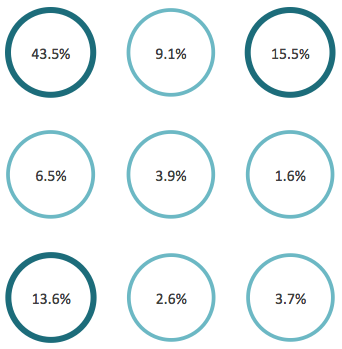
\includegraphics[width=0.45\textwidth]{pics/analysis/RRT.png}
          \label{fig:handednessstartingpoint1}
        }
        \hspace{0.5cm}
        \subfigure[Patterns created by right-handed respondents holding the smartphone in the left hand using the forefinger on the left hand]{
          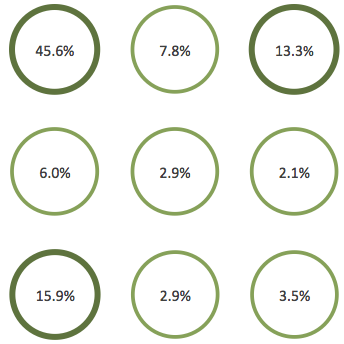
\includegraphics[width=0.45\textwidth]{pics/analysis/RLF.png}
          \label{fig:handednessstartingpoin2}
        }
        \subfigure[Patterns created by left-handed respondents holding the smartphone in the left hand using the thumb on the same hand]{
          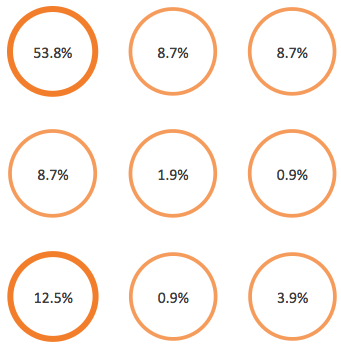
\includegraphics[width=0.45\textwidth]{pics/analysis/LLT.png}
          \label{fig:handednessstartingpoint3}
        }
        \hspace{0.5cm}
        \subfigure[Patterns created by left-handed respondents holding the smartphone in the right hand using the forefinger on the left hand]{
          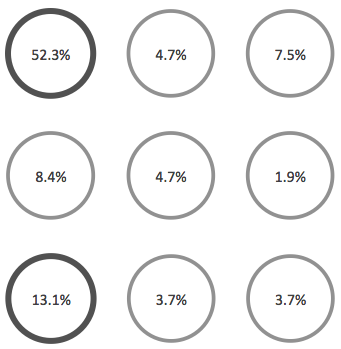
\includegraphics[width=0.45\textwidth]{pics/analysis/LRF.png}
          \label{fig:handednessstartingpoint4}
        }
        \caption{Starting node based on handedness, hand used to hold smartphone, and finger used used when creating patterns}
        \label{fig:handednessstartingpoint}
      \end{figure}

  \clearpage
	\subsection{Experience with IT and Security}

  \todo[inline, color=blue!60]{Kanskje sette kjønn opp mot erfaring pga det er flere gutter som har erfaring med IT og sikkerhet. Hvis gutter lager bedre mønster er dette også fordi de har mer erfaring med IT/Sikkerhet? Kanskje skille på jenter og gutter uten erfaring for sammenligning?}

  This section takes a more detailed review of the patterns created by people with different experience with IT and security. The level of interest and experience with IT and security can cause people to create different passwords based on risk and security awareness. 

    \subsubsection{Average pattern creation time}

      Figure \ref{fig:avgcreationtimeexperience} is showing the average creation time measured in seconds for both respondents experienced and respondents not experienced with IT and security. 

      Figure \ref{fig:avgcreationtimeyes} are showing the average creation time for the three pattern types created by respondents experienced with IT and security. The patterns with the highest creation time is the patterns created for banking accounts with an average creation time of 9.42 seconds. The patterns with the lowest average creation time are created for smartphones with an average creation time of 7.75 seconds.

      Figure \ref{fig:avgcreationtimeno} are showing the average creation time for the three pattern types created by respondents unexperienced with IT and security. The patterns with the highest creation time is the patterns created for banking accounts with an average creation time of 9.29 seconds. The patterns with the lowest average creation time are created for smartphones with an average creation time of 7.42 seconds.

      Comparing the experienced and unexperienced respondents, the unexperienced respondents has a slightly lower response time for pattern creation for all three pattern types. 

      %Figure: Average pattern creation time for Experience
      \begin{figure}[H]
        \centering
        \subfigure[Experience with IT and security]{
          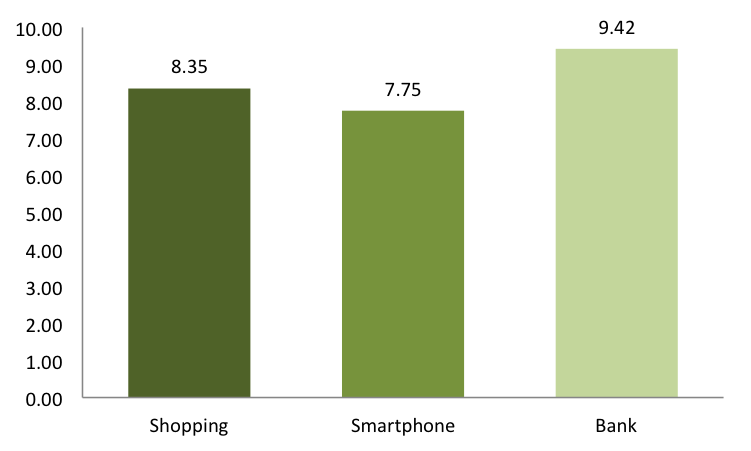
\includegraphics[width=0.45\textwidth]{pics/analysis/creationtime-experience-yes.png}
          \label{fig:avgcreationtimeyes}
        }
        \subfigure[No experience with IT and security]{
          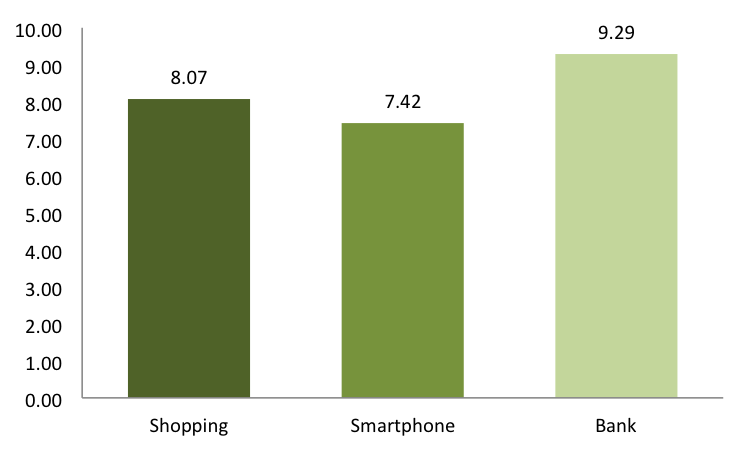
\includegraphics[width=0.45\textwidth]{pics/analysis/creationtime-experience-no.png}
          \label{fig:avgcreationtimeno}
        }
        \caption{Average pattern creation time for experience with IT and security}
        \label{fig:avgcreationtimeexperience}
      \end{figure}

    \subsubsection{Average pattern length}

      Figure \ref{fig:avgpatternlengthexperience} are showing the average pattern length for patterns created by both respondents experienced and unexperienced with IT and security.

      Figure \ref{fig:avgpatternlengthyes} are showing the average pattern length for patterns created by respondents experienced with IT and security. The patterns with the highest average pattern length are created for banking accounts with a total average pattern length of 6.11. The pattern type with the shortest average pattern length are patterns created for smartphones with an average pattern length of 5.48.

      Figure \ref{fig:avgpatternlengthfeno} are showing the average pattern length for patterns created by respondents unexperienced with IT and security. The patterns with the highest average pattern length are created for banking accounts with a total average pattern length of 5.61. The pattern type with the shortest average pattern length are patterns created for smartphones with an average pattern length of 5.27. 

      The tendencies in the graphs shows that respondents with experience in IT and security have a longer patterns than people unexperienced with IT and security for all three pattern types. For both graphs, patterns created for banking accounts has the highest average length, while patterns created for smartphones have the shortest average pattern length. 

      %Figure: Average pattern length for experience
      \begin{figure}[H]
        \centering
        \subfigure[Experience with IT and security]{
          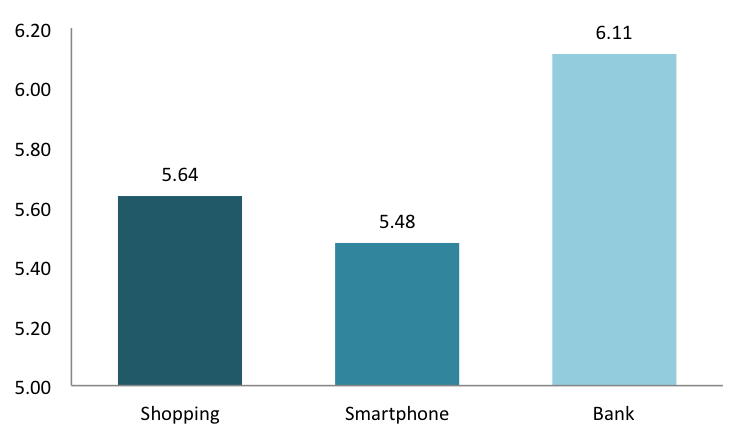
\includegraphics[width=0.45\textwidth]{pics/analysis/avgpatternlength-experience-yes.png}
          \label{fig:avgpatternlengthyes}
        }
        \subfigure[No experience with IT and security]{
          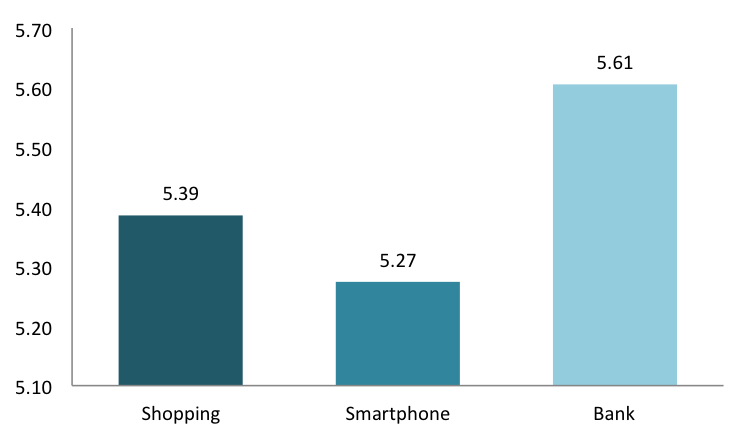
\includegraphics[width=0.45\textwidth]{pics/analysis/avgpatternlength-experience-no.png}
          \label{fig:avgpatternlengthfeno}
        }
        \caption{Average pattern length for experience with IT and security}
        \label{fig:avgpatternlengthexperience}
      \end{figure}

    \subsubsection{Pattern length distribution}

      Figure \ref{fig:avgpatterndistexperience} is showing the distribution of pattern length based on the respondents experience with IT and Security for all pattern types. 

      Figure \ref{fig:avgpatternlengthdistyes} is the pattern length distribution of patterns created by respondents experienced with IT and security. The patterns created for smartphoens, 70\% of the patters constitutes of patterns with a lower length, e.g. patterns with a length of 4 to 6 nodes. For patterns created for banking accounts, 62\% of the patterns are created with a lower length. The patterns with length 9, the maximum length of a pattern, have the highest frequency of patterns created for banking accounts. 

      Figure \ref{fig:avgpatternlengthdistno} is the pattern length distribution of patterns created by respondents unexperienced with IT and security. The patterns created for smartphoens, 79\% of the patters constitutes of patterns with a lower length, e.g. patterns with a length of 4 to 6 nodes. For patterns created for banking accounts, 70\% of the patterns are created with a lower length.

      By comparing the pattern length distribution of both experienced and unexperienced respondents in Figure \ref{fig:avgpatternlengthdistyes} and \ref{fig:avgpatternlengthdistno}, respectively, the patterns created by unexperienced respondents have a higher frequency of patterns with lower pattern length than patterns created by experienced respondents. The the most distinct difference is that experienced respondents creates less patterns of low length for banking accounts than unexperienced respondents, instead they have a higher frequency of patterns with length 9 for banking accounts. Experienced users do only have 27\% of their patterns for banking accounts created with the length 4, while unexperienced users have about 39\% of their patterns for banking accounts created with the length 4. 

      Both graphs shows that the lower the length the lower the frequency will occur. The only exception is patterns of length 8 that breaks the descending pattern of the plot. 

      %Figure: Average pattern length distribution for experience
      \begin{figure}[H]
        \centering
        \subfigure[Experience with IT and security]{
          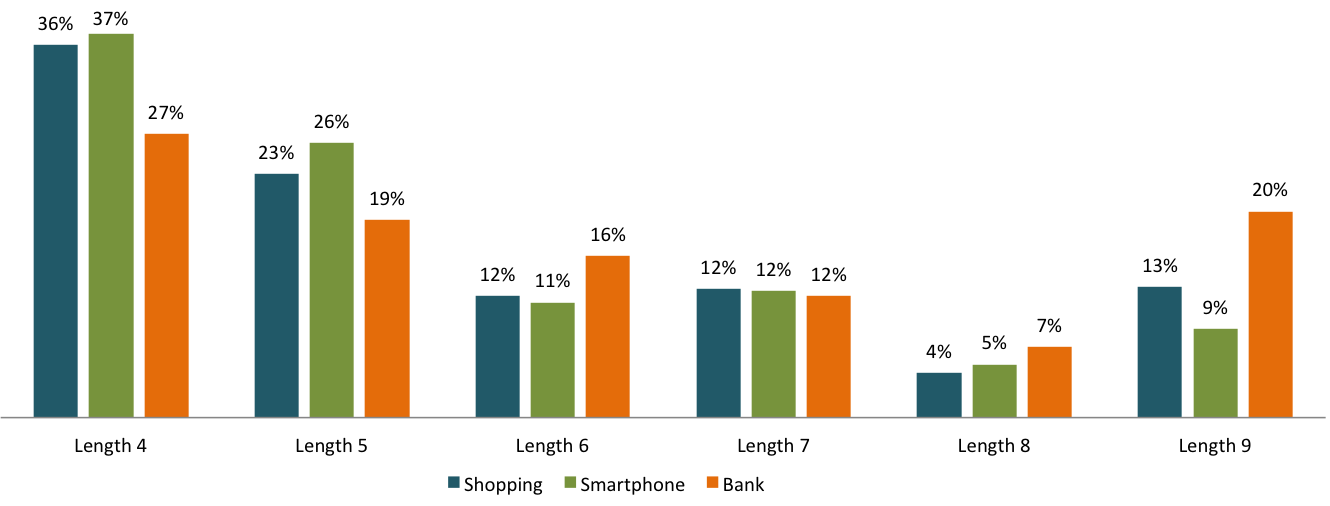
\includegraphics[width=1.0\textwidth]{pics/analysis/patterndist-experience-yes.png}
          \label{fig:avgpatternlengthdistyes}
        }
        \subfigure[No experience with IT and security]{
          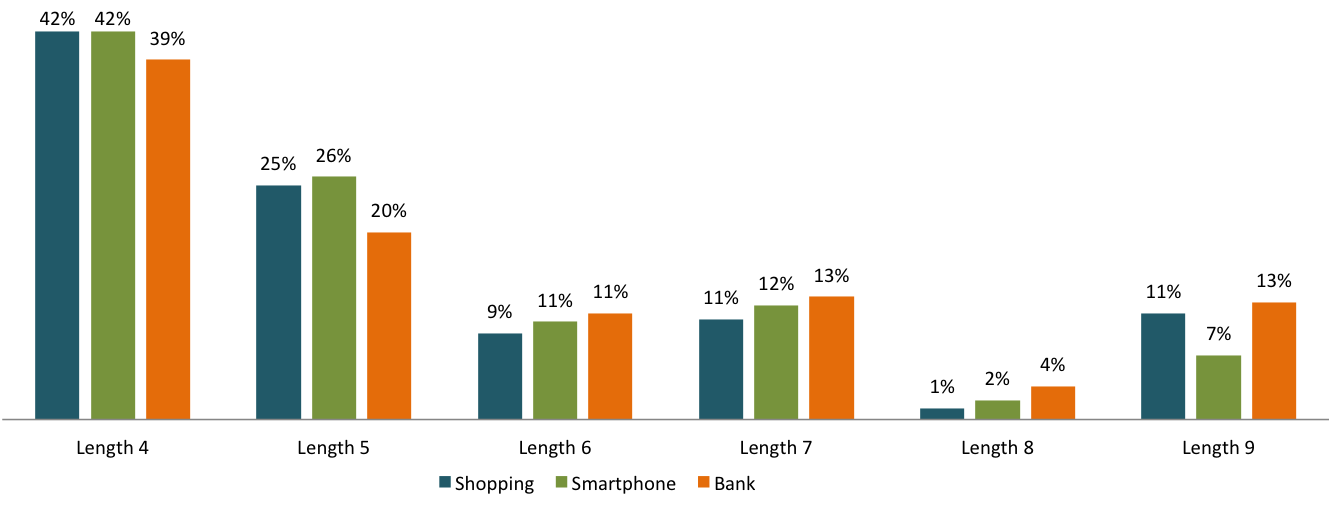
\includegraphics[width=1.0\textwidth]{pics/analysis/patterndist-experience-no.png}
          \label{fig:avgpatternlengthdistno}
        }
        \caption{Average pattern length distribution for experience with IT and security}
        \label{fig:avgpatterndistexperience}
      \end{figure}

    \subsubsection{Pattern complexity}

      Table \ref{tab:experiencestrength} is the pattern strength for each pattern type with respect to the experience with IT and security for the respondents, including a overview of the parameters used to calculate the pattern strength. 
 

      % INTERSECTION
      %- On average 35\% mindre intersections  

      % OVERLAPS

      % TOTAL STRENGTH

      % MIN AND MAXIMUM STRENGTH

      %Table: Password strength and Experience with IT/Security
      \begin{table}[H]
        \centering
        \begin{tabular}{l || l | l || l | l || l | l }
          \hline
           & \multicolumn{2}{c||}{\bf Shopping} & \multicolumn{2}{c||}{\bf Smartphone} &\multicolumn{2}{c}{\bf Bank} \\ \hline
          {\bf Parameters}   & {\bf Yes} & {\bf No} & {\bf Yes} & {\bf No} & {\bf Yes} & {\bf No}\\ \hline
          \#Patterns         & 470    & 332    & 470    & 332    & 470    & 332    \\
          Avg. Size          & 5.636  & 5.386  & 5.479  & 5.274  & 6.113  & 5.605  \\
          Avg. Length        & 5.182  & 4.818  & 5.045  & 4.753  & 5.919  & 5.281  \\
          \#Intersections    & 123    & 41     & 108    & 34     & 231    & 121    \\
          Avg. Intersections & 0.262  & 0.123  & 0.230  & 0.102  & 0.491  & 0.364  \\
          \#Overlaps         & 10     & 4      & 9      & 3      & 13     & 6      \\
          Avg. Overlaps      & 0.021  & 0.012  & 0.019  & 0.009  & 0.028  & 0.018  \\ \hline
          Avg. Strength      & 13.911 & 12.635 & 13.271 & 12.202 & 16.417 & 14.089 \\ 
          Min strength       & 6.340  & 6.340  & 6.340  & 6.340  & 6.340  & 6.340  \\
          Max strength       & 44.441 & 39.827 & 43.187 & 38.870 & 44.441 & 44.441 \\ \hline
        \end{tabular}
        \caption{Password strength and Experience with IT/Security}
        \label{tab:experiencestrength} 
      \end{table}

